%\documentclass[../document.tex]{subfiles}
%\begin{document}

\chapter{Support Vector Machines}

Verranno ora approfondite le tematiche brevemente introdotte nel \textbf{Capitolo 1} riguardo l'apprendimento supervisionato, focalizzando l'attenzione sulle \textit{SVM} --- \textit{Support Vector Machine}, \textit{macchine a vettori di supporto}.

La fase di apprendimento di tale tipologia di classificatori è basata su considerazioni di tipo geometrico, ed in particolare sul concetto di \textit{iperpiano di separazione}.
Verrà dapprima analizzato il caso banale in cui i dati di \textit{training} siano linearmente separabili, per poi generalizzare i concetti presentati al caso \textit{soft-margin}. Saranno infine introdotte le funzioni \textit{kernel}, ponendo l'attenzione sul modo in cui quest'ultime si integrano nel formalismo delle \textit{SVM}.

\section{Dati linearmente separabili}

\paragraph{Interpretazione geometrica}
Si introduce la trattazione delle \textit{SVM} nel caso più semplice da illustrare: si supponga inizialmente che i dati del \textit{training set} da cui ottenere la funzione di decisione ricercata siano \textit{linearmente separabili} \cite{vapnik}.

\paragraph{}
Sia $T$ un \textit{training set} --- come definito nel \textbf{Capitolo 1} --- costituito da $n$ coppie ordinate:
\begin{equation}
T = \left\{ { (\boldsymbol{x}_i, y_i);\; i = 1, 2 \;...\; n;\; \boldsymbol{x}_i \in \mathbb{R}^d; \; y_i \in \left\{-1, +1\right\} }\right\}.
\end{equation}

La prima componente della $i$-esima coppia è l'osservazione $\boldsymbol{x}_i$, rappresentata come un \\* \textit{punto} in uno spazio continuo $d$-dimensionale ($X \in \mathbb{R}^d$). Ogni osservazione consta quindi di $d$ componenti, o \textit{feature}. La seconda componente della $i$-esima coppia rappresenta l'etichetta di classe $y_i$ --- nota a priori --- associata alla osservazione $\boldsymbol{x_i}$. 

Poiché $C = \left\{ -1, +1 \right\}$ risulta evidente come si stia trattando un problema si classificazione \textit{binario}, ovvero con $k = |C| = 2$ classi. Denotiamo allora con
\begin{equation}
	T_+ = \left\{ \boldsymbol{x}_+ \in \mathbb{R}^d \;|\; (\boldsymbol{x}_+, +1) \in T \right\}	
\end{equation}
\begin{equation}
	T_- = \left\{ \boldsymbol{x}_- \in \mathbb{R}^d \;|\; (\boldsymbol{x}_-, -1) \in T \right\}		
\end{equation}

rispettivamente la \textit{classe dei positivi} e la \textit{classe dei negativi}.

\paragraph{}
L'idea fondamentale alla base della classificazione mediante \textit{SVM} è quella di separare geometricamente le due classi (e per estensione i rispettivi punti) ricorrendo a un \textit{iperpiano di separazione}.
Ricordiamo che un \textit{iperpiano} in $\mathbb{R}^d$ è così definito:
\begin{equation}
	H = \left\{ x \in \mathbb{R}^d \,|\, w \cdot x + b = 0;\; w \in \mathbb{R}^d \right\}
\end{equation}

ovvero come un insieme di punti $x$ che soddisfano una equazione lineare caratterizzata dai coefficienti $w$ e $b$, dove: $w$ è un vettore ortogonale (\textit{normale}) all'iperpiano $H$ (e indica la sua direzione), $b$ è il termine noto (spesso indicato in letteratura come \textit{offset} o \textit{bias}).

Ricordiamo inoltre che un iperpiano è una generalizzazione della nozione intuitiva di \textit{piano} su spazi $d$-dimensionali con $d \neq 2,\, d \neq 3$; i.e. per $d = 1$ un iperpiano è rappresentato da un punto in un dato spazio uni-dimensionale, per $d = 2$ è una retta in uno spazio bi-dimensionale, per $d = 3$ è un piano (nella comune accezione del termine) in uno spazio tri-dimensionale, e così via.

\begin{figure} %%% FIGURA A
 	\centering	
	
	\fboxsep=0mm%padding thickness
	\fboxrule=1mm%border thickness

	\fcolorbox{border_color}{white} {
		\includegraphics[scale=1]{img/FiguraA_ScatterPN.eps}
		%\includegraphics[scale=1]{../img/FiguraA_ScatterPN.eps}
	}	
	\caption{Due classi di punti positivi ($T_+$) e negativi ($T_-$) in $\mathbb{R}^2$ (scatter plot)}
\end{figure}

\begin{figure} %%% FIGURA B
 	\centering	
	
	\fboxsep=0mm%padding thickness
	\fboxrule=1mm%border thickness

	\fcolorbox{border_color}{white} {
		\includegraphics[scale=1]{img/FiguraB_PNconIperpiano.eps}
		%\includegraphics[scale=1]{../img/FiguraB_PNconIperpiano.eps}
	}	
	\caption{Tre iperpiani di separazione in $\mathbb{R}^2$ (rette), con dati linearmente separabili}
\end{figure}

\paragraph{}
Un iperpiano possiede la desiderabile proprietà di dividere i rimanenti punti dello spazio in due \textit{semispazi} (semirette, semipiani, etc.) disgiunti. La strategia adoperata consiste dunque nell'individuare un iperpiano adatto alla costruzione di una funzione di decisione, al fine di classificare osservazioni successive. In prima istanza, si richiede l'\textit{esistenza} di un iperpiano in grado di bipartire lo spazio $\mathbb{R}^d$ in \textit{semispazio positivo} (contenente \textit{solamente} i punti di $T_+$) e \textit{semispazio negativo} (contenente \textit{solamente} i punti di $T_-$).

Un tale iperpiano è detto \textit{di separazione}.
Fissato quindi un \textit{dataset} $T$ avente rispettive classi $T_+$ e $T_-$, se esiste un iperpiano di separazione per tali insiemi di punti si dice che essi sono \textit{linearmente separabili}.
In accordo a quanto mostrato nella sezione successiva, si chiarisce sin d'ora che la separabilità lineare non è strettamente necessaria per la costruzione di classificatori basati su \textit{SVM}: essa rappresenta infatti una condizione molto restrittiva, difficilmente soddisfatta in \textit{dataset} provenienti da applicazioni reali.

Ai fini della trattazione, si assumerà al momento che tale ipotesi irrealistica sia verificata.

\paragraph{}
Posto che gli insiemi di punti $T_+$ e $T_-$ siano linearmente separabili, ci si propone si trovare per essi un iperpiano di separazione. Risulta evidente l'esistenza di un numero infinito di tali iperpiani: un criterio di scelta ragionevole prevede di selezionare il particolare iperpiano di separazione \textit{a massimo margine}.

Sia $H$ un qualunque iperpiano di separazione, $d_+$ ($d_-$) la distanza euclidea fra $H$ e il più vicino positivo $\boldsymbol{x_+} \in T_+$ (negativo $\boldsymbol{x_-} \in T_-$), banalmente calcolata ricorrendo alla formula 

\begin{equation}
	d_+ = d(\boldsymbol{x_+}, H) = \frac{|w \cdot \boldsymbol{x_+} + b|}{||w||}
	\vspace{2mm}
\end{equation}

\vspace{2mm} dove $||w||$ è la norma euclidea $\sqrt{w_1^2 + ... + w_d^2} \;$ (analogo per $\boldsymbol{x_-}$).

Si definisce il \textit{margine} di un iperpiano di separazione $H$ la quantità $d_+ + d_-$.

\begin{figure} %%% FIGURA C
 	\centering	
	
	\fboxsep=0mm%padding thickness
	\fboxrule=1mm%border thickness

	\fcolorbox{border_color}{white} {		
		\includegraphics[scale=0.9]{img/FiguraC_margine.eps}
		%\includegraphics[scale=1]{../img/FiguraC_margine.eps}
	}	
	\caption{Iperpiano di separazione a massimo margine $H_M$ in $\mathbb{R}^2$}
\end{figure}

\paragraph{}
Il problema si traduce quindi nella ricerca di valori dei coefficienti $w$ e $b$ tali che --- fra tutte le possibili scelte di $w$ e $b$ --- essi permettano di ottenere l'iperpiano $H_M$ di separazione con margine $d_+ + d_-$ massimo.
\begin{equation}
	H_M:  w \cdot \boldsymbol{x} + b = 0 \;.
\end{equation}

Si supponga adesso di scegliere opportunamente un fattore di scala per $w$ e $b$ in modo che risultino vere, per l'ipotesi di separabilità lineare, le seguenti asserzioni:
\begin{equation}
	w \cdot \boldsymbol{x_i} + b \geq +1 \;\; \mbox{per} \;\; y_i = +1, \;\; \forall \; i = 1, 2 \;...\; n
\end{equation}
\begin{equation}
	w \cdot \boldsymbol{x_i} + b \leq -1 \;\; \mbox{per} \;\; y_i = -1, \;\; \forall \; i = 1, 2 \;...\; n
\end{equation}
(una per ogni elemento in $T$), riscrivibili in forma compatta come:
\begin{equation}
	y_i(w \cdot \boldsymbol{x_i} + b) -1 \geq 0, \;\; \forall \; i = 1, 2 \;...\; n \;.
\end{equation}
Allo scopo di inquadrare visivamente il significato geometrico del problema, si considerino inoltre due iperpiani ausiliari $H_+$ e $H_-$, così definiti:
\begin{equation}
	H_+: w \cdot \boldsymbol{x} + b = +1
\end{equation}
\begin{equation}
	H_-: w \cdot \boldsymbol{x} + b = -1 \; .
\end{equation}

È evidente che $H_+$ e $H_-$ sono paralleli (poiché hanno lo stesso $w$) e differiscono per il termine noto.
Inoltre, entrambi risultano paralleli all'iperpiano ricercato $H_M$.

L'insieme di vincoli (2.7) indica che gli esempi positivi ($\boldsymbol{x} \in T_+$), come si illustra in Figura C, sono posizionati nell'area ``al di sopra'' dell'iperpiano $H_+$, o eventualmente vi appartengono. Ciò equivale a dire che \textit{nessun} positivo oltrepassa $H_+$ dal lato opposto.
La stessa considerazione si applica --- a segni inversi --- con la (1.8) agli esempi negativi. In definitiva, tutte le condizioni (2.9) impongono che nessuno dei punti di \textit{training} sia ricada nell'area compresa fra $H_+$ e $H_-$.
I punti $\boldsymbol{x_+}$ e $\boldsymbol{x_-}$ (quelli più vicini, appartenenti a classi distinte) giacciono proprio su $H_+$ e $H_-$, rispettivamente. È da notare inoltre che l'iperpiano ricercato $H_M$ sia posizionato esattamente ``a metà strada'' fra $H_+$ e $H_-$.

\paragraph{}
Si consideri adesso un qualsiasi punto $\boldsymbol{x_h} \in H_M$; dalle riflessioni appena fatte segue che il margine è ricavabile come la misura della distanza fra gli iperpiani $H_+$ e $H_-$. La distanza $d_+$ tra il punto $\boldsymbol{x_h}$ e l'iperpiano $H_+$ è:

\begin{equation}
	d_+ = \frac{| \boldsymbol{x_h} \cdot w + (b - 1) |}{||w||}
	\vspace{2mm}
\end{equation}

analogamente, la distanza $d_-$ tra il punto $\boldsymbol{x_h}$ e l'iperpiano $H_-$ è:

\begin{equation}
	d_- = \frac{| \boldsymbol{x_h} \cdot w + (b + 1) |}{||w||}
	\vspace{2mm}
\end{equation}
%\vspace{2mm}


Ma poiché $\boldsymbol{x_h} \in H$, vale $\boldsymbol{x_h} \cdot w + b = 0$.
\\ In definitiva, un'espressione per il margine è data da

\begin{equation}
	d_+ + d_- = \frac{|-1|}{||w||} + \frac{|1|}{||w||} = \frac{2}{||w||} \; .
\end{equation}

\paragraph{}

L'addestramento di una \textit{SVM} coincide in pratica con la risoluzione del seguente problema di ottimizzazione: massimizzare la funzione obiettivo $2 / ||w||$ sotto i vincoli dati da (2.9), nelle variabili $w$ e $b$. Ciò equivale a minimizzare $||w|| / 2$ sotto le stesse condizioni. Per semplicità verrà considerata invece la funzione obiettivo $||w||^2 / 2$, con
\begin{equation}
	||w||^2 = \left( \sqrt{w_1^2 + ... + w_d^2} \right)^2 = w_1^2 + ... + w_d^2 = w \cdot w
\end{equation}
la cui soluzione --- sempre rispetto ai vincoli (2.9) --- è la medesima. In questo modo viene eliminato lo svantaggio computazionale derivante dal calcolo di una radice quadrata. Il fattore di $1 / 2$ è similmente mantenuto per convenienza matematica (durante i calcoli).

\paragraph{}
Più formalmente, ci si pone in definitiva il seguente problema:
\begin{equation}	
\begin{split}
	&\argmin {w, b} { \frac{1}{2} ||w||^2 }
	\\ &y_i(w \cdot \boldsymbol{x_i} + b) -1 \geq 0, \;\; \forall \; i = 1, 2 \;...\; n \;.
\end{split}
\end{equation}

\paragraph{}
I punti $\boldsymbol{x_s}$ che appartengono a $H_+$ o a $H_+$ sono detti \textbf{vettori di supporto} (\textit{support vectors}, da qui il nome del modello); una loro eventuale rimozione dal \textit{training set} cambia la soluzione del problema di ottimizzazione.
Secondo le definizioni date in precedenza, $\boldsymbol{x_+}$ e $\boldsymbol{x_-}$ sono \textit{dei} vettori di supporto: è infatti ammissibile l'esistenza di più punti giacenti sugli iperpiani $H_+$ e $H_+$; segue che il numero di vettori di supporto può essere $s > 2$. 

Rimuovere dal \textit{training set} un qualsiasi punto --- sia esso positivo o negativo --- che non fa parte dei vettori di supporto non influenza invece la soluzione trovata (ovvero i valori desiderati di $w$ e $b$).

\paragraph{Ottimizzazione}
Si accennerà ora alla formulazione del suddetto problema di ottimizzazione; la traccia della seguente discussione è ispirata a \cite{tutorial}.

Si consideri la forma Lagrangiana del problema --- ottenuta applicando quindi il metodo dei moltiplicatori di Lagrange alla funzione obiettivo $||w||^2 / 2$ --- la quale permette di semplificare la notazione di esso, operando con vincoli meglio trattabili.

Siano $n$ moltiplicatori di Lagrange positivi $\alpha_i \in \mathbb{R}, \; i = 1, 2\; ... \;n $; uno per ciascuna delle $n$ condizioni in (2.9) (ovvero uno per ogni elemento del \textit{training set}).
Ricordiamo che, per vincoli della forma $c_i \geq 0$, il metodo prevede di sottrarre alla funzione obiettivo le espressioni dei vincoli moltiplicate ai coefficienti positivi $\alpha_i \geq 0$.
Ciò conduce alla forma:
\begin{equation}
\vspace{2mm}
 	L_P = \frac{1}{2}||w||^2 - \sum\limits_{i = 1}^{n} {\lbrack \alpha_i y_i (w \cdot \boldsymbol{x_i} + b) - 1 \rbrack}
\vspace{2mm}
\end{equation}

dove il pedice $P$ in $L_P$ indica che il problema è espresso in forma primale. 
\paragraph{}
Il problema di ottimizzazione è quindi stato trasformato nella equivalente formulazione: minimizzare $L_P$ rispetto a $w$ e $b$, imponendo che $\alpha_i \geq 0$ e richiedendo che le $i$ derivate parziali $\partial L_p / \partial \alpha_i$ si annullino --- si denoti questo insieme di vincoli con $C_1$. Esso risulta essere un problema di programmazione quadratica convesso, visto che (a) la funzione obiettivo $L_P$ è convessa (b) l'insieme dei punti che soddisfano i vincoli (i.e. l'insieme ammissibile) è un insieme convesso (poiché ogni vincolo lineare della (2.9) descrive un insieme convesso e l'intersezione di $n$ insiemi convessi è ancora un insieme convesso).

\paragraph{}
Ciò permette di passare ad una formulazione duale del problema (nota come ``duale di Wolfe''): \textit{massimizzare} $L_P$ (sempre rispetto a $w$ e $b$) imponendo che $\alpha_i \geq 0$ e richiedendo stavolta che siano le derivate parziali $\partial L_P / \partial w$ e $\partial L_P / \partial b$ ad annullarsi --- si denoti questo insieme di vincoli $C_2$.
La formulazione primale e quella duale sono equivalenti: la minimizzazione di $L_P$ rispetto ai vincoli $C_1$ e la massimizzazione di $L_P$ rispetto ai vincoli $C_2$ conducono alla stessa soluzione (ovvero agli stessi valori di $w$ e $b$).

\paragraph{}
Dai vincoli sulle derivate parziali in $C_2$
\begin{equation}	
	\frac{\partial L_P}{\partial w} = 0
\end{equation}
\begin{equation}	
	\frac{\partial L_P}{\partial b} = 0
	\vspace{2mm}
\end{equation}
derivando $L_P$ nei due casi e risolvendo, si trova rispettivamente:
\begin{equation}		
	w = \sum\limits_{i = 1}^{n} {\alpha_i y_i \boldsymbol{x_i}}
\end{equation}
\begin{equation}
	\sum\limits_{i = 1}^{n} {\alpha_i y_i} = 0
\vspace{2mm}
\end{equation}
e sostituendo nella (2.17) si ottiene da $L_P$ una espressione per $L_D$:
\begin{equation}
	L_D = \sum\limits_{i = 1}^{n} {\alpha_i} - \frac{1}{2} \sum\limits_{\substack{i = 1 \\ j = 1}}^{N} {\alpha_i \alpha_j y_i y_j \; \boldsymbol{x_i} \cdot \boldsymbol{x_j}}
\end{equation} 
dove il pedice $D$ in $L_D$ indica che il problema è espresso nella sua forma duale.

\paragraph{}
Come già affermato, $L_P$ e $L_D$ corrispondono a problemi di ottimizzazione differenti (sia in termini di funzione obiettivo sia di vincoli) ma che conducono alla stessa soluzione. È da notare in particolare come nella (2.22) non figuri più la dipendenza dalle variabili $w$ e $b$, quanto piuttosto dai moltiplicatori $\alpha_i$. La fase di \textit{training} di una \textit{SVM} è quindi sintetizzabile, in ultima istanza, come la massimizzazione di $L_D$ rispetto ai coefficienti $\alpha_i$.

Sebbene sia presente un moltiplicatore $\alpha_i$ per ciascun punto di training $\boldsymbol{x_i}$, generalmente la maggior parte di essi sarà nullo: vale infatti che $\alpha_i > 0$ (strettamente positivo) solo per i vettori di supporto (che indicheremo d'ora in poi con $\boldsymbol{x_s} \in SV$).
Ciò è coerente con quanto affermato dalla espressione (2.20) --- la quale fornisce un modo diretto per ricavare il valore di $w$ ricercato --- dove è evidente come i punti $\boldsymbol x \not\in SV$ non incidano nel calcolo della soluzione trovata.
I vettori di supporto sono dunque gli elementi critici del \textit{training set}, dalla cui entità dipende direttamente il calcolo della funzione di decisione $f$. 

\paragraph{}
Nonostante sia stata ricavata una espressione immediata per il calcolo di $w$, l'iperpiano di separazione a massimo margine ricercato non è ancora univocamente determinato --- non è ancora noto infatti il valore di $b$.
Di seguito si fornisce una espressione per ricavare $b$ a partire dalle condizioni di Karush-Kuhn-Tucker.

\paragraph{Condizioni di Karush-Kuhn-Tucker}
Tali condizioni rivestono un ruolo fondamentale sia nella teoria che nella pratica della risoluzione di problemi di ottimizzazione vincolata. Essendo una loro trattazione teorica ben oltre gli scopi di questo elaborato, ne verrà fornita una presentazione concisa e non esaustiva.

Riguardo il particolare caso affrontato nei paragrafi precedenti, per il problema di ottimizzazione espresso in forma primale $L_P$ valgono le seguenti condizioni:

\begin{equation}
	\frac{\partial}{\partial w_j} L_P = w_j - \sum\limits_{i = 1}^{n} {\alpha_i y_i x_{ij}} = 0 \;\;\; \forall \; j = 1, 2, \;...\; d
\end{equation}
\begin{equation}
	\frac{\partial}{\partial b} L_P = - \sum\limits_{i = 1}^{n} {\alpha_i \boldsymbol{x_i}} = 0
\end{equation}
\begin{equation}
	y_i(w \cdot \boldsymbol{x_i} + b) - 1 \geq 0 \;\;\; \forall \; i = 1, 2, \;...\; n
\end{equation}
\begin{equation}
	\alpha_i \geq 0 \;\;\; \forall \; i = 1, 2, \;...\; n\end{equation}
\begin{equation}
	\alpha_i(y_i(w \cdot \boldsymbol{x_i} + b) - 1) = 0 \;\;\; \forall \; i = 1, 2, \;...\; n \;.
\vspace{2mm}
\end{equation}
che risultano essere soddisfatte dalla soluzione del problema di ottimizzazione. Inoltre, in presenza di problemi convessi --- ed è questo il caso --- tali condizioni risultano essere \textit{necessarie e sufficienti} affinché $w$, $b$ e gli $\alpha_i$ siano soluzioni del problema.
Si utilizzi, per lo scopo preposto, il vincolo (2.27) detto ``condizione di complementarità''. Esso consente di ricavare di $b$ a partire dalla conoscenza di $w$ e di almeno un vettore di supporto. Riscrivendo $b$ in forma esplicita si ha:
\begin{equation}
	b = \frac{1}{y_i} - w \cdot \boldsymbol{x_s} \;\;\; 
\vspace{2mm}
\end{equation}
comunque scelto $\boldsymbol{x_s} \in SV$ (ovvero un qualsiasi vettore di supporto).
È comunque buona pratica (adottata peraltro in sistemi automatici che implementano il \textit{training} \textit{SVM}) calcolare un $b_i$ per ogni vettore di supporto ed assumere come valore definitivo la media dei $b_i$ ottenuti, in modo da ovviare ad inesattezze derivanti da approssimazioni intermedie nel calcolo di $b$.

\paragraph{Test}
Una volta ricavati sia $w$ che $b$, non rimane che esplicitare la funzione di decisione $f$ da utilizzare per predire le etichette di osservazioni successive in input. $f$ è quindi fortemente legata all'iperpiano di separazione a massimo margine identificato dai coefficienti $w$ e $b$. L'espressione finale per $f$ è data da:
\begin{equation}
	f(\boldsymbol{x}; w, b) = sign(w \cdot \boldsymbol{x} + b)
\end{equation}
dove banalmente si classifica $\boldsymbol{x}$ a seconda della sua posizione rispetto all'iperpiano $H_M$.

Nel corso del \textbf{Capitolo 3} verrà mostrato come alcune tecniche di estensione di classificatori binari (quindi \textit{SVM}) al caso multiclasse richiedano la conoscenza di informazioni ulteriori rispetto alla sola etichetta predetta (i.e. la distanza dell'osservazione $\boldsymbol{x}$ dall'iperpiano $H_M$, utilizzata come \textit{score}, ``punteggio'').

%%%%%%%%%%%%%%%%%%%%%%%%%%%%%%%%%%%%%%%%%%%%%%%%%%%%%%%%%%%%%%%%%%%%%%%%%%%%%%%%%%%%%%%%%%%%%%%%%%%%

\section{Dati non linearmente separabili}

\paragraph{Interpretazione geometrica}
Ci si ponga adesso nel caso in cui i punti in $T_+ \cup T_-$ \textit{non} siano linearmente separabili, ovvero non esista alcun iperpiano $H$ di separazione tale che i semispazi da esso individuati contengano esclusivamente punti di una sola classe.
Questo è ovviamente lo scenario più comune nei casi in cui si abbia a che fare con \textit{dataset} provenienti da applicazioni reali (e non meramente didattici).

\begin{figure}[H] %%% FIGURA D
 	\centering	
	
	\fboxsep=0mm%padding thickness
	\fboxrule=1mm%border thickness

	\fcolorbox{border_color}{white} {
		\includegraphics[scale=1]{img/FiguraD_nonseparabili.eps}
		%\includegraphics[scale=1]{../img/FiguraD_nonseparabili.eps}
	}	
	\caption{Due classi di punti non linearmente separabili in $H_M$ in $\mathbb{R}^2$}
\end{figure}

Sotto queste ipotesi, non valgono le considerazioni fatte nella sezione precedente per la ricerca di una soluzione al problema di ottimizzazione quadratica, visto che esse dipendevano dall'insieme di vincoli (2.9) --- i quali non sono più verificati.
Il meccanismo, in questo caso, consiste nel riformulare il problema originario così da consentire la presenza di ``errori'' in fase di \textit{training}, ovvero di quei punti la cui presenza determina la non-separabilità delle classi. Un classificatore \textit{SVM} addestrato in questo modo cercherà comunque di ottenere la separazione più ``pulita'' possibile, cercando ancora una volta di massimizzare la separazione fra $T_+$ e $T_-$.

\paragraph{}
Al fine di ottenere un tale classificatore, si introducano $n$ variabili ausiliarie di \textit{slack} positive $\xi_i \geq 0$; $i = 1, 2 \; ... \; n \;$ (una per ogni elemento di \textit{training}), in modo da riscrivere i vincoli (2.9) nella nuova forma:
\begin{equation}
	w \cdot \boldsymbol{x_i} + b \geq +1 - \xi_i \;\; \mbox{per} \;\; y_i = +1, \;\; \forall \; i = 1, 2 \;...\; n
\end{equation}
\begin{equation}
	w \cdot \boldsymbol{x_i} + b \leq -1 + \xi_i \;\; \mbox{per} \;\; y_i = -1, \;\; \forall \; i = 1, 2 \;...\; n \;.
\end{equation}

\begin{figure}[H] %%% FIGURA E
 	\centering	
	
	\fboxsep=0mm%padding thickness
	\fboxrule=1mm%border thickness

	\fcolorbox{border_color}{white} {
		\includegraphics[scale=0.9]{img/FiguraE_soft.eps}		
		%\includegraphics[scale=1]{../img/FiguraE_soft.eps}
	}	
	\caption{$\boldsymbol{x_E}$ è un punto ``in errore'' poiché è situato oltre l'iperpiano $H_S$}
	%Si noti che la sua distanza da $H_-$ è $\xi_E / ||w||$}
\end{figure}

Si supponga di aver trovato un iperpiano $H_S$ per tale problema di separazione.
Si osservi che --- come indicato in figura B --- affinché si verifichi un errore per $\boldsymbol{x}_E$ il rispettivo $\xi_E$ associato debba essere maggiore di 1 (e.g. se $\boldsymbol{x}_E$ è un positivo, ricade nel semispazio negativo individuato da $H_S$; ovvero la distanza tra $\boldsymbol{x}_E$ e $H_+$ deve essere superiore al margine). 
Gli $\xi_i$ rappresentano quindi dei coefficienti di penalità associati ai punti; e per quanto detto prima la somma degli $n$ $\xi_i$ è una limitazione superiore al numero di punti di errore in fase di \textit{training}.

\paragraph{}
Si desidera dunque trovare un iperpiano in modo tale massimizzare il margine di separazione fra le due classi (la distanza tra i due iperpiani $H_+$ e $H_-$ paralleli ad $H_S$ e passanti rispettivamente per $\boldsymbol{x_+}$ e $\boldsymbol{x_-}$, i più vicini punti non affetti da errore), cercando al contempo di minimizzare l'errore complessivo commesso.

La funzione obiettivo da minimizzare adatta allo scopo è:
\begin{equation}
	\frac{||w||^2}{2} + C \left( \sum\limits_{i = 1}^{n} {\xi_i} \right)^k
\vspace{2mm} 
\end{equation}
dove $C$, scelto dall'utente, controlla la penalità associata all'errore. % Tale funzione rappresenta in definitiva la ricerca di un compromesso fra un grande margine e una piccola penalità di errore. 
Per ogni intero positivo $k$ il problema risulta essere ancora convesso; e per $k = 1$ o $k = 2$ è ancora un problema di programmazione quadratica.

\paragraph{}
Fatte le considerazioni analoghe al caso linearmente separabile, $L_P$ diventa:
\begin{equation}
 	L_P = \left[ \frac{||w||^2}{2} + C \left( \sum\limits_{i = 1}^{n}{\xi_i} \right)^k \right]  	
 	- \sum\limits_{i = 1}^{n} {\left[ \alpha_i y_i (w \cdot \boldsymbol{x_i} + b) - 1 + \xi_i \right]}  	
 	- \sum\limits_{i = 1}^{n} { \mu_i \xi_i } 		
\vspace{2mm}
\end{equation}
dove i $\mu_i \geq 0$ sono gli $n$ ulteriori moltiplicatori di Lagrange relativi alle variabili $\xi_i$.
La scelta di $k = 1$ ha il vantaggio che, nel passaggio alla forma duale del problema, né gli $\xi_i$ né i coefficienti $\mu_i$ compaiono in $L_p$, che rimane:
\begin{equation}
	L_D = \sum\limits_{i = 1}^{n} {\alpha_i} - \frac{1}{2} \sum\limits_{\substack{i = 1 \\ j = 1}}^{N} {\alpha_i \alpha_j y_i y_j \; \boldsymbol{x_i} \cdot \boldsymbol{x_j}}
\end{equation} 
soggetta alla ulteriore condizione:

\begin{equation}	
	\frac{\partial L_P}{\partial \xi_i} = C - \alpha_i - \mu_i = 0
	\vspace{2mm}
\end{equation}
da cui $\alpha_i = C - \mu_i$, e poiché $\mu_i \geq 0$, si ha $ \alpha_i \leq C$.
In definitiva, l'unica differenza rispetto alla formulazione orginaria è che il vincolo sui moltiplicatori $\alpha_i$ è adesso $0 \leq \alpha_i \leq C$. Questa formulazione del problema è anche detta \textit{soft-margin} \cite{cortes}.

\paragraph{}
Per brevità, verranno omesse le condizioni di Karush-Kuhn-Tucker relative al nuovo $L_P$, delle quali si può trovare un elenco in \cite{tutorial}. Ci si limiterà a dire, in questa sede, che la condizione di complementarità per il calcolo di $b$ assume la forma:
\begin{equation}
	\alpha_i(y_i(w \cdot \boldsymbol{x_i} + b) - 1 + \xi_i) = 0 \;\;\; \forall \; i = 1, 2, \;...\; n \;.
\end{equation}
da cui:
\begin{equation}	
	b = \frac{1 - \xi_i}{y_i} - w \cdot \boldsymbol{x_s} \;\;\; 
\vspace{2mm}
\end{equation}
per la quale valgono le stesse considerazioni del caso linearmente separabile.

Risolto il nuovo problema di ottimizzazione e trovati $w$ e $b$ opportuni, la fase di test è analoga al caso precedente.

%%%%%%%%%%%%%%%%%%%%%%%%%%%%%%%%%%%%%%%%%%%%%%%%%%%%%%%%%%%%%%%%%%%%%%%%%%%%%%%%%%%%%%%

\section{Funzioni kernel e SVM non lineari}

L'estensione del \textit{training} \textit{SVM} al caso \textit{soft-margin} si propone di rimediare al caso in cui i punti su cui operare non siano perfettamente separabili tramite un iperpiano. Tuttavia sono comuni i casi in cui, \textit{non solo} essi \textit{non} sono linearmente separabili, ma in aggiunta presentano configurazioni più complesse; cosicché ha poco senso cercare di separarli ricorrendo ad iperpiani. Si veda un esempio in Figura F, che illustra graficamente il problema in $\mathbb{R}^2$.

\begin{figure}[H] %%% FIGURA F
 	\centering	
	
	\fboxsep=0mm%padding thickness
	\fboxrule=1mm%border thickness

	\fcolorbox{border_color}{white} {
		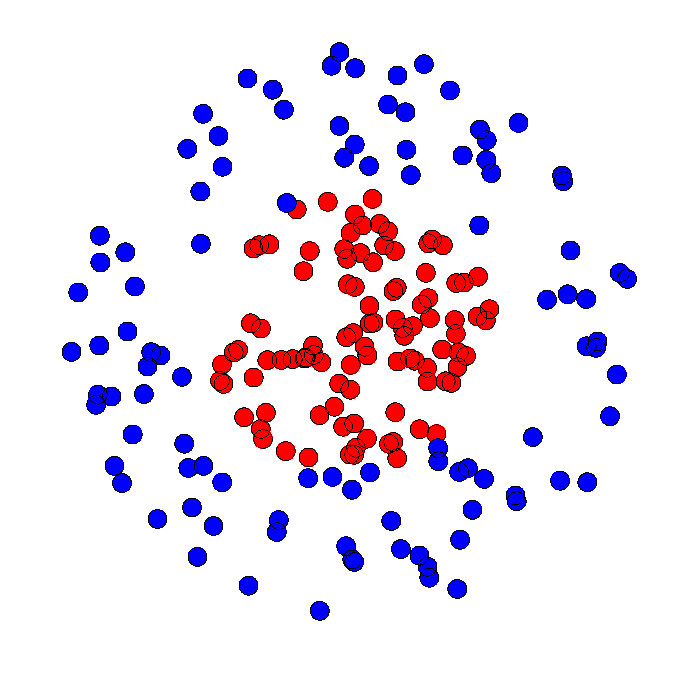
\includegraphics[scale=0.9]{img/circular.eps}		
		%\includegraphics[scale=1]{../img/FiguraE_soft.eps}
	}	
	\caption{Due classi non linearmente separabili in $\mathbb{R}^2$}
	%Si noti che la sua distanza da $H_-$ è $\xi_E / ||w||$}
\end{figure}
\paragraph{}
Il modo in cui tale problematica viene elegantemente ed efficacemente affrontata dalle \textit{SVM} è uno dei punti di forza a favore del loro utilizzo in applicazioni pratiche. L'idea di base è la seguente: si supponga di conoscere una funzione $\phi$ che trasforma i punti $\boldsymbol{x}_i$, mappandoli dal loro dominio $T_+ \cup T_-$ (lo spazio dei dati) ad uno spazio $F$ (lo spazio delle \textit{feature}) a dimensione maggiore. Sia quindi $\phi$:
\begin{equation}
\begin{split}
	\phi : & D \subseteq \mathbb{R}^d \longrightarrow F \subseteq \mathbb{R}^m
	\\& x \longmapsto \phi(x)
\end{split}
\end{equation}
con $m > d$. L'intuizione è quella di separare \textit{non} i punti $\boldsymbol{x_i}$ con un iperpiano in $\mathbb{R}^d$, quanto piuttosto le immagini $\phi(\boldsymbol{x_i})$ con un iperpiano in $F$; dove esse risultano più facilmente (e in alcuni casi linearmente) separabili. Ciò significa che punti soggetti al problema di ottimizzazione \textit{non} sono gli $x_i$ ma i relativi $\phi(\boldsymbol{x_i})$. Per predire l'etichetta di una nuova osservazione  $\boldsymbol{x}$, è necessario valutare quindi la posizione di  $\phi({\boldsymbol{x}})$ rispetto all'iperpiano di separazione che risiede nello spazio delle features $F$.

\paragraph{}
Questo approccio sembra ragionevole, ma presenta uno svantaggio: osservando le equazioni che caratterizzano il problema di ottimizzazione --- e in particolare la (2.22) --- si intuisce come la fase di addestramento sia basata fondamentalmente sul calcolo di prodotti scalari del tipo $\phi(\boldsymbol{x_i}) \cdot \phi(\boldsymbol{x_j})$ (essendo i dati mappati in $F$ prima di effettuare l'ottimizzazione). Poiché $F$ ha in genere un elevato numero di dimensioni, ciò comporta che la fase di addestramento può risultare computazionalmente pesante da effettuare.
Tale potenziale inefficienza è aggirata facendo uso del cosiddetto \textbf{kernel trick} \cite{aizerman}.

\paragraph{}
Si consideri la funzione
$\phi(x_1, x_2) = (x_1^2, \sqrt{2} x_1 x_2, x_2^2)$ la quale mappa un punto $x \in \mathbb{R}^2$ ($x_1$ e $x_2$ sono le sue componenti) nello spazio $\mathbb{R}^3$ (si assume al momento per semplicità di trattazione che $m$ non sia molto grande).

Si calcoli il prodotto scalare $\phi(\boldsymbol{x}) \cdot \phi(\boldsymbol{y})$:
\begin{equation}
\begin{split}
	\phi(\boldsymbol{x}) \cdot \phi(\boldsymbol{y}) &= (x_1^2, \sqrt{2}x_1 x_2, x_2^2) \cdot (y_1^2, \sqrt{2}y_1 y_2, y_2^2) 
	\\ &= x_1^2 y_1^2 + 2 x_1 x_2 y_1 y_2 + x_2^2 y_2^2
	\\ &= (x_1 y_1 + x_2 y_2)^2
	\\ &= \left( (x_1, x_2) \cdot (y_1, y_2) \right) ^ 2 = (\boldsymbol{x} \cdot \boldsymbol{y}) ^ 2 \;. 
\end{split}
\end{equation}
Si evince, dai passaggi sopraelencati, come sia stato ricavato un modo per calcolare il suddetto prodotto scalare senza dover ricorrere necessariamente al calcolo esplicito di $\phi$, e quindi di dover operare all'interno dello spazio $F$, con le sue numerose $m$ componenti.
\paragraph{}
Il ``trucco'' (letteralmente, \textit{trick}) consiste quindi nell'individuare una \textbf{funzione kernel} $K$ tale che $K(\boldsymbol{x}, \boldsymbol{y}) = \phi(\boldsymbol{x}) \cdot \phi(\boldsymbol{y})$, ovvero una differente espressione per il calcolo del prodotto scalare che consenta di ottenere tale valore senza ``passare'' per $\phi$.

Il kernel $K_2 = (\boldsymbol{x} \cdot \boldsymbol{y}) ^ 2 $ utilizzato nel precedente esempio è detto kernel \textit{quadratico}; una sua generalizzazione è data dal kernel \textit{polinomiale} $K_p = (\boldsymbol{x} \cdot \boldsymbol{y}) ^ p$. Sebbene nell'esempio fornito non sia immediatamente evidente l'alta dimensionalità di $F$ si consideri che, dato $K_p$, la $\phi$ associata produce una esplosione combinatoria del numero di dimensioni in $F$, che risulta uguale a \cite{bing2011} \cite{tutorial}
\begin{equation}
	\binom {d + p -1} {p}
	\vspace{2mm}
\end{equation}

\paragraph{}
Per quanto riguarda le \textit{SVM}, fissato appositamente un kernel $K$ (la sui scelta deriva da un'analisi dei dati da trattare), è possibile sostituire $K(\boldsymbol{x}, \boldsymbol{y})$ ovunque si presenti di un prodotto scalare del tipo $\phi(\boldsymbol{x}) \cdot \phi(\boldsymbol{y})$. Si consideri ad esempio il calcolo della funzione di decisione (2.29) in presenza di una trasformazione $\phi$:
\begin{equation}
\begin{split}
	f(\boldsymbol{x}; w, b) &= sign(w \cdot \boldsymbol{x} + b)
	\\ & = sign\left( \left( \sum\limits_{i = 1}^{n}{\alpha_i y_i \phi(\boldsymbol{x_i})} \right) \cdot \phi(\boldsymbol{x}) + b\right)
	\\ & = sign\left( \sum\limits_{i = 1}^{n}{\alpha_i y_i \phi(\boldsymbol{x_i}) \cdot \phi(\boldsymbol{x}) } + b\right)
	\\ & = sign\left( \sum\limits_{i = 1}^{n}{\alpha_i y_i K(\boldsymbol{x_i}, \boldsymbol{x}) } + b\right)
\end{split}
\vspace{2mm}
\end{equation}

Notare come in tale formulazione sia possibile predire l'etichetta dell'osservazione $\boldsymbol{x}$ senza ricavare direttamente il valore di $w$. Verrà ripreso un ragionamento simile nel \textbf{Capitolo 3}, quando si manifesterà il problema di dover calcolare la distanza tra $\boldsymbol{x}$ e l'iperpiano di separazione in $F$; con $w$ incognito.

\paragraph{}
Per avere un'idea visuale di come agisce il kernel nello spazio dei dati, si veda la Figura G, la quale mostra che, data la natura non lineare di $\phi$, all'iperpiano nello spazio delle \textit{features} vi corrisponde una superficie di separazione (\textit{decision boundary}). Essa, a differenza di quanto succede nel caso lineare (e.g con una retta in $\mathbb{R}^2$, si presta meglio nell'adattarsi --- in un certo senso --- alla forma delle classi.
Il kernel utilizzato in questo caso --- e negli esperimenti del \textbf{Capitolo 4} --- è:
\begin{equation}
	K(\boldsymbol{x}, \boldsymbol{y}) = e^{-\frac{||\boldsymbol{x} - \boldsymbol{y}||^2}{2\sigma^2}}
\end{equation}
noto come \textit{RBF} kernel (\textit{radial basis function}, funzione a base radiale) \cite{tutorial}.

\begin{figure}[H] %%% FIGURA F
 	\centering	
	
	\fboxsep=0mm%padding thickness
	\fboxrule=1mm%border thickness

	\fcolorbox{border_color}{white} {
		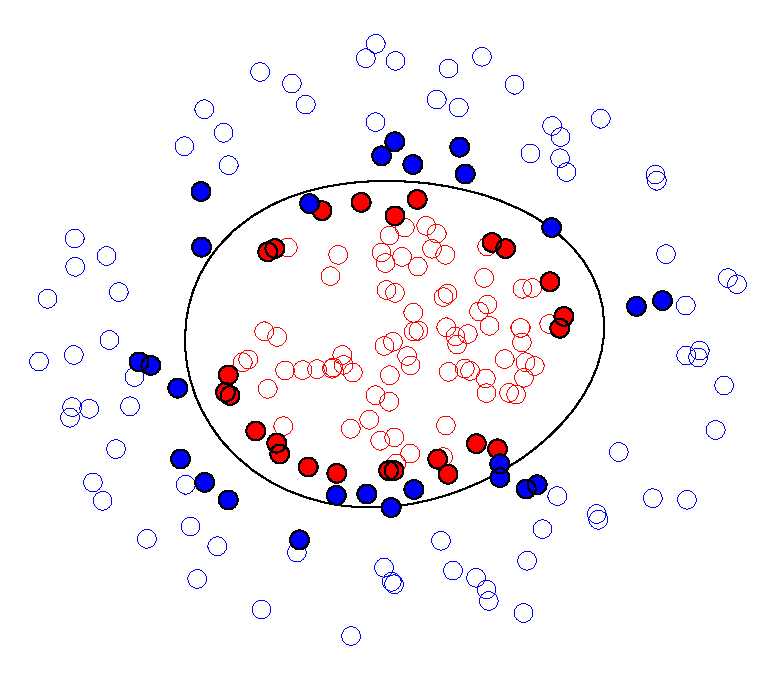
\includegraphics[scale=1]{img/rbfkern.eps}		
		%\includegraphics[scale=1]{../img/FiguraE_soft.eps}
	}	
	\caption{Decision boundary per due classi non linearmente separabili in $\mathbb{R}^2$, identificato tramite kernel rbf. Sono evidenziati i vettori di supporto}
	%Si noti che la sua distanza da $H_-$ è $\xi_E / ||w||$}
\end{figure}

\paragraph{}
È inoltre importante notare come il kernel \textit{trick} non si applichi solamente alle \textit{SVM}, ma potenzialmente a tutti i metodi che fanno uso di prodotti scalari nella suddetta forma (si parla così di \textit{metodi kernel}). Per una trattazione approfondita di tali applicazioni, si veda \cite{kernels}.

%%%%%%%%%%%%%%%%%%%%%%%%%%%%%%%%%%%%%%%%%%%%%%%%%%%%%%%%%%%%%%%%%%%%%%%%%%%%%%%%%%%%%%%%%%%%%

\section{Ulteriori considerazioni}

\paragraph{Complessità}
Nel completare infine la presentazione delle \textit{SVM}, oggetto di questo capitolo, verranno esposte alcune considerazioni relative al loro utilizzo in applicazioni reali. Il nucleo dell'utilizzo delle \textit{SVM} risiede nella risoluzione del problema di programmazione quadratica già discusso; esistono numerose librerie e dei pacchetti software per l'ottimizzazione vincolata (\textit{general purpose}) che, in casi semplici (ovvero per \textit{dataset} di dimensione contenuta) danno risultati soddisfacenti.

Quando la dimensione del problema da risolvere è grande, occorrono tecniche più raffinate per poter lavorare sui dati in modo efficiente. Discutere dell'implementazione concreta di suddette tecniche SVM va ben oltre gli scopi del presente lavoro; si accenna in questa sede solo al fatto che alcuni algoritmi dedicati operano suddividendo i dati in sottoproblemi (si veda ``\textit{chunking}'') rendendo il \textit{training} parallelizzabile. \cite{tutorial}

In genere, la complessità computazionale di tali algoritmi si colloca fra $O(n^3)$ e $O(n^2)$ \cite{tutorial}. Per quanto riguarda il \textit{testing} di una singola osservazione si ha invece, nel caso banale, una complessità di $O(k s)$, dove $k$ indica il numero di operazioni effettuate nella valutazione del kernel $K$ scelto, $s$ è il numero di vettori di supporto --- vedasi la (2.41). Nel caso lineare, dove $w$ è calcolabile esplicitamente (senza ricorrere a $K$) dopo l'addestramento, la complessità di \textit{testing} si riduce invece a $O(1)$.

\paragraph{Implementazioni}
Fra le implementazioni che si ritengono maggiormente degne di nota (in quanto più popolari) vi sono: \textit{LIBSVM} \footnote{http://www.csie.ntu.edu.tw/~cjlin/libsvm/} (una libreria \textit{open-source} scritta in C++ e \textit{portata} su un'innumerevole quantità di linguaggi e piattaforme), SVMLight \footnote{http://svmlight.joachims.org/}, scikit-learn \footnote{http://scikit-learn.org/stable/} (framework per \textit{machine learning} in Python), WEKA \footnote{http://www.cs.waikato.ac.nz/ml/weka/} (software per \textit{machine learning} scritto in Java), e infine le API dello \textit{Statistics Toolbox} presente in \textit{MATLAB} \footnote{http://www.mathworks.it/it/help/stats/support-vector-machines.html} (la cui \textit{Student Version r2014a} è stata utilizzata per lo sviluppo di questa tesi). Una lista di implementazioni si trova in \cite{userguide}.

\paragraph{Svantaggi}
Come già fatto presente, la fase di training può essere computazionalmente lenta quando si trattano dati dalla grande entità (si immagini di avere a che fare con \textit{dataset} di milioni di elementi). In tali casi, non è quindi da trascurare neanche il costo in termini di memoria occupata, sia in fase di training che di testing --- in virtù di quanto detto prima, se il kernel è non lineare, occorre memorizzare tutti i vettori di supporto per il calcolo di $f$.

Le \textit{performance} di classificazione di una \textit{SVM} sono inoltre fortemente legate alla scelta del kernel, che può essere difficile da identificare. Tutto ciò ricordando sempre che una \textit{SVM} può solamente essere utilizzata in presenza di $k = 2$ classi. Esistono comunque lavori volti a generalizzare le \textit{SVM} per la gestione del caso multiclasse secondo un approccio \textit{single machine}, ovvero risolvendo un unico problema di ottimizzazione (quindi un singolo \textit{training}) per tutte le $k$ classi \cite{tutorial}. Nel corso del \textbf{Capitolo 3} si tratteranno invece metodi per l'estensione di classificatori binari al caso multiclasse tramite aggregazione di più ``macchine'' (approccio certamente più semplice).

%\end{document}